\documentclass[serif,mathserif]{beamer}
\usepackage{amsmath, amsfonts, epsfig, xspace}
\usepackage{algorithm,algorithmic}
\usepackage{pstricks,pst-node}
\usepackage{multimedia}
\usepackage[normal,tight,center]{subfigure}
\setlength{\subfigcapskip}{-.5em}
\usepackage{beamerthemesplit}
\usepackage{../beamerthemelankton-keynote}

\author[Joe Rocklin]{Joe Rocklin\\@joerocklin}

\title[Lesson 01\hspace{2em}\insertframenumber/\inserttotalframenumber]{Lesson 01 - What is Software}

\date{September 15, 2015} %leave out for today's date to be insterted

\institute{Siemens PLM Software}

\begin{document}

\maketitle

% \section{Introduction}  % add these to see outline in slides

\begin{frame}
  \frametitle{Introduction}
  Joe Rocklin
  \begin{columns}[T]
  \begin{column}[T]{.5\textwidth}
    \begin{itemize}
    \item Milford HS, 2000
    \item Univeristy of Cincinnati\\B.S. Computer Science 2005
    \item University of Cincinnati\\Graduate studies in Computer Engineering
    \end{itemize}
  \end{column}
  \pause
  \begin{column}[T]{.5\textwidth}
    \begin{itemize}
    \item Co-Op at SDRC, MeadWestvaco, Cinergy, and UC Research
    \item Northrop Grumman, 2005-2012
    \item Siemens PLM, 2012-Present
    \item HTG, LLC 2006-Present
    \end{itemize}
  \end{column}
  \end{columns}
\end{frame}

\begin{frame}{Areas of Interest}
  \begin{itemize}
  \item Operating Systems
  \item Hardware/Software Interactions
  \item Distributed Systems
  \item Security
  \item Education
  \end{itemize}
\end{frame}

\section{What is Software} % add these to see outline in slides

\begin{frame}{What it Software?}
  Software is a set of machine-readable instructions which directs a processor to perform specific actions.
\end{frame}

\subsection{Processors}

\begin{frame}{Processors}
  Three main tasks:
  \begin{itemize}
  \item<1-> Fetch \only<2->{ - Read an instruction from memory}
  \item<1-> Decode \only<3->{ - Figure out what the instruction is}
  \item<1-> Execute \only<4->{ - Do whatever the instruction says to do}
  \end{itemize}
\end{frame}

\begin{frame}{Memory}
  Memory Heirarchy
  \begin{itemize}
  \item<1-> Hard Drives \only<2->{ - Terrabytes or more}
  \item<3-> RAM \only<4->{ - 10's - 100's of Gigabytes}
  \item<5-> Cache\only<7->{\footnote{Based on Intel Skylake series processors, announced August 2015}} \only<6->{ - On the processor silcon directly}
    \begin{itemize}
    \item<7-> L3 \only<8->{ - 8192KiB shared}
    \item<7-> L2 \only<8->{ -  256KiB per core}
    \item<7-> L1 \only<8->{ -   64KiB per core}
    \end{itemize}
  \item<9-> Registers
  \end{itemize}
\end{frame}

\begin{frame}{Processor}
  \begin{figure}
  \centering
  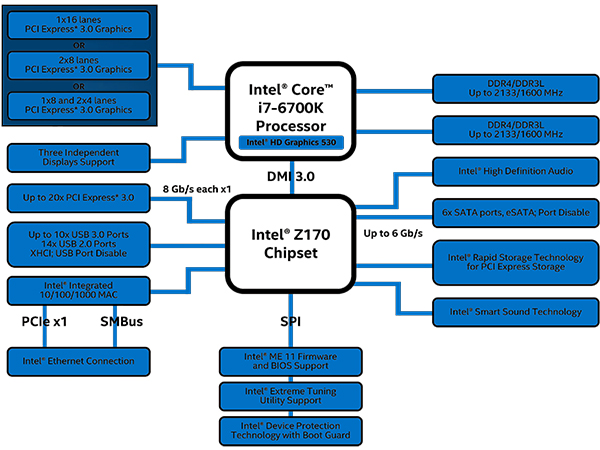
\includegraphics[height=0.75\textheight]{Intel-Z170-chipset-block-diagram.jpg}
  \caption{Intel Z170 Chipset Block Diagram}
  \label{fig:intel-z170-chipset}
  \end{figure}
\end{frame}

% \begin{frame}
%   \frametitle{Pictures}
%   \begin{figure}[t]
%     \centering
%     \subfigure[First Frame]{
% %    \includegraphics[width=3cm]{figures/naked_leaves/00000001}}
%     \includegraphics[width=3cm]{lion.png}}
%     \subfigure[Middle Frame]{
% %    \includegraphics[width=3cm]{figures/naked_leaves/00000120}}
%     \includegraphics[width=3cm]{lion.png}}
%     \subfigure[Last Frame]{
% %    \includegraphics[width=3cm]{figures/naked_leaves/00000240}}
%     \includegraphics[width=3cm]{lion.png}}
%   \end{figure}
% \end{frame}
%
% \begin{frame}
%   \frametitle{A Movie}
%   \begin{center}
%     \movie[height=5cm,width=6.5cm,poster,autostart,loop]{}{leaves.avi}
%   \end{center}
%   \begin{itemize}
%   \item Movies only seem to work in Adobe Reader
%   \item Movie file is not embedded, it must be on the computer
%   \end{itemize}
% \end{frame}
%
% % \section{Conclusion} % add these to see outline in slides
%
% \begin{frame}
%   \frametitle{Credits}
%   \begin{itemize}
%   \item Brought to you by www.shawnlankton.com
%   \item Please let me know about improvements!
%   \item This was supposed to look like a KeyNote Show
%   \item inspiration: http://www.ucl.ac.uk/~ucbpeal/latexposter.html
%   \item inspiration: http://newsgroups.derkeiler.com/... (in code)
%         %http://newsgroups.derkeiler.com/Archive/Comp/comp.text.tex/2007-11/msg00299.html
%   \end{itemize}
% \end{frame}

\begin{frame}
  \frametitle{Questions}
\end{frame}
\end{document}
